\documentclass[a4paper,12pt,twoside,brazilian,english]{book}
\usepackage{imegoodies}
\usepackage[thesis]{imelooks}
\usepackage{lipsum}

\graphicspath{{figuras/},{fig/},{logos/},{img/},{images/},{imagens/}}

\addbibresource{bibliografia.bib}

\title{Título do trabalho}[um subtítulo]
\translatedtitle{Title of the document}[a subtitle]

\author[mas]{Antonio Fernando Silva e Cruz Filho \\ João Gabriel Andrade de Araujo Josephik}


\def\profa{Prof\kern.02em.\kern-.07emª\kern.07em}
\def\dra{Dr\kern-.04em.\kern-.11emª\kern.07em}

\orientador[fem]{Prof. Nina S. T. Hirata}

\banca{
    \profa{} \dra{} Fulana de Tal (orientadora) -- IME-USP [sem ponto final],
    % Em inglês, não há o "ª"
    %Prof. Dr. Fulana de Tal (advisor) -- IME-USP [sem ponto final],
    Prof. Dr. Ciclano de Tal -- IME-USP [sem ponto final],
    \profa{} \dra{} Convidada de Tal -- IMPA [sem ponto final],
}

\tipotese{
  %mestrado,
  %doutorado,
  tcc,
  %definitiva, % É a versão para defesa ou a versão definitiva?
  %quali, % É qualificação?
  programa={Ciência da Computação},
}

\defesa{
  local={São Paulo},
  data=2017-08-10, % YYYY-MM-DD
}

\direitos{CC-BY}

\fichacatalografica{}  % n sei pra que isso serve. Por enquanto ...


\begin{document}

%%%%%%%%%%%%%%%%%%%%%%%%%%% CAPA E PÁGINAS INICIAIS %%%%%%%%%%%%%%%%%%%%%%%%%%%%

\frontmatter

\pagestyle{plain}

\onehalfspacing % Espaçamento 1,5 na capa e páginas iniciais

\maketitle % capa e folha de rosto

%%%%%%%%%%%%%%%% DEDICATÓRIA, AGRADECIMENTOS, RESUMO/ABSTRACT %%%%%%%%%%%%%%%%%%


% Reinicia o contador de páginas (a próxima página recebe o número "i") para
% que a página da dedicatória não seja contada.
\pagenumbering{roman}

\chapter*{Agradecimentos}
\epigrafe{Do. Or do not. There is no try.}{Mestre Yoda}

Texto texto texto texto texto texto texto texto texto texto texto texto texto
texto texto texto texto texto texto texto texto texto texto texto texto texto
texto texto texto texto texto texto texto texto texto texto texto texto texto
texto texto texto texto. Texto opcional.

%!TeX root=../tese.tex
%("dica" para o editor de texto: este arquivo é parte de um documento maior)
% para saber mais: https://tex.stackexchange.com/q/78101

% As palavras-chave são obrigatórias, em português e em inglês, e devem ser
% definidas antes do resumo/abstract. Acrescente quantas forem necessárias.
\palavraschave{IA, Aprendizado de Máquina, IA Explicável, XAI, Visualização de Características, GradCam, LIME}

\keywords{AI, Machine Learning, Explainable AI, XAI, Feature visualization, GradCam, LIME}

% O resumo é obrigatório, em português e inglês. Estes comandos também
% geram automaticamente a referência para o próprio documento, conforme
% as normas sugeridas da USP.
\resumo{
Com a ascensão do uso de Aprendizado de Máquina para problemas de Visão Computacional, o uso de Redes Neurais Convolucionais (CNNs) se mostrou uma peça fundamental para a criação de modelos estado da arte em tarefas como classificação, detecção de objetos e até mesmo segmentação.
No entanto,em muitos casos, a simples obtenção do resultado de uma predição não é suficiente, sendo necessária uma justificativa para as decisões do modelo.
Utilizando IA Explicável (XAI), podemos encontrar possíveis explicações para predições de modelos complexos como Redes Convolucionais. 
Nesse trabalho, foram estudadas diversas técnicas de Explicabilidade aplicadas a CNNs, utilizando de técnicas como GradCam e Visualização de Características. 
Além disso, foram conduzidos experimentos com cada técnica abordada visando avaliar a eficácia na interpretação dos modelos de Visão Computacional.
}

\abstract{
With the rise of Machine Learning in Computer Vision problems, the use of Convolutional Neural Networks (CNNs) has proven to be a fundamental component in developing state-of-the-art models for tasks such as classification, object detection, and even segmentation.
However, in many cases, simply obtaining the result of a prediction is not sufficient; a justification for the model's decisions is necessary.
By employing Explainable AI (XAI), it is possible to identify potential explanations for the predictions of complex models such as Convolutional Neural Networks.
In this study, various explainability techniques applied to CNNs were analyzed, utilizing methods such as Grad-CAM and Feature Visualization.
Additionally, experiments were conducted with each technique to assess their effectiveness in interpreting Computer Vision models.
}


%%%%%%%%%%%%%%%%%%%%%%%%%%% LISTAS DE FIGURAS ETC. %%%%%%%%%%%%%%%%%%%%%%%%%%%%%

% Settings importantes definidos pelo pessoal do github que administra os templates
\cleardoublepage

\newcommand\disablenewpage[1]{{\let\clearpage\par\let\cleardoublepage\par #1}}

\bgroup
\raggedbottom

%%%%% Listas criadas manualmente

%\chapter*{Lista de abreviaturas}
\disablenewpage{\chapter*{List of Abbreviations}}

\begin{tabular}{rl}
   AI  & Artificial Intelligence \\
   XAI & Explainable AI \\
   MLP & Multilayer Perceptron \\
   CNN & Convolutional Neural Network \\
   Conv & Convolution \\
   IME & Institute of Mathematics and Statistics\\
   USP & University of São Paulo
\end{tabular}

% Quebra de página manual
\clearpage

%%%%% Listas criadas automaticamente

% Você pode escolher se quer ou não permitir a quebra de página
%\listoffigures
\disablenewpage{\listoffigures}

% Você pode escolher se quer ou não permitir a quebra de página
%\listoftables
\disablenewpage{\listoftables}

% Esta lista é criada "automaticamente" pela package float quando
% definimos o novo tipo de float "program" (em utils.tex)
% Você pode escolher se quer ou não permitir a quebra de página
%\listof{program}{\programlistname}
\disablenewpage{\listof{program}{\programlistname}}

% Sumário (obrigatório)
\tableofcontents

\egroup % Final de "raggedbottom"

%%%%%%%%%%%%%%%%%%%%%%%%%%%%%%%% CAPÍTULOS %%%%%%%%%%%%%%%%%%%%%%%%%%%%%%%%%%%%%

\mainmatter

\pagestyle{mainmatter}

% Espaçamento simples
\singlespacing

% A introdução não tem número de capítulo, então os cabeçalhos também não
\pagestyle{unnumberedchapter}

% Capitulos:
%!TeX root=../tese.tex
%("dica" para o editor de texto: este arquivo é parte de um documento maior)
% para saber mais: https://tex.stackexchange.com/q/78101

%% ------------------------------------------------------------------------- %%

% "\chapter" cria um capítulo com número e o coloca no sumário; "\chapter*"
% cria um capítulo sem número e não o coloca no sumário. A introdução não
% deve ser numerada, mas deve aparecer no sumário. Por conta disso, este
% modelo define o comando "\chapter**".

% Falar na introdução:

% É bom deixar isso para o final, com o proj. completo.

% começar explicando o crescimento de redes neurais, ia e inteligência artificial 
% nos últimos tempos, da importância de redes convolucionais e o quão perigoso 
% elas podem ser por conta de sua natureza "desconhecida", já que são modelos 
% explicáveis e não interpretáveis. 

% Explicar a importância de se justificar decisões de modelos em situações do mundo real 
% e como pode ser prejudicial a deficiência disso 

% Chegar em um foco para imagens em especial, falando que existem ferramentas/métodos que ajudam a 
% avaliar decisões de redes neurais,  dando segurança para usuários.

% Como fazer citação: \citet{(ccódigo de citação)} para citação direta
% e \citep{(ccódigo de citação)} para citação por entre parênteses.

% Use \emph para enfatizar texto e \textit para texto em itálico.

\chapter**{Introduction}
\label{chap:introduction}

\enlargethispage{.5\baselineskip}

\lipsum[1-2]

\section**{Other Section Example}
\label{sec:consideracoes_preliminares}

\lipsum[3-4]

\section**{Next Section example}

\lipsum[5-7]

%!TeX root=../tese.tex
%("dica" para o editor de texto: este arquivo é parte de um documento maior)
% para saber mais: https://tex.stackexchange.com/q/78101

% Aqui podemos começar falando um pouco sobre o background de explainable AI e depois conectamos
% falando sobre redes neurais e gradiente descendente para, por fim, falar um pouco sobre CNNs.


\enlargethispage{-1\baselineskip}

\chapter{Background}

In this chapter, we will introduce important concepts required for the understanding of this study.
We begin by introducing Explainable AI (XAI) and its principles. We also introduce Neural Networks and important concepts such as Gradient Descent and Back Propagation. 
Finally, we introduce Convolutional Neural Networks, the main focus of this study.

\section{Explainable AI}

With the rise of Machine Learning models in the last decade in the business and academic areas, Artificial Intelligence (AI) is becoming increasingly present in important decision-making tasks. 
However, as AI models have become more sophisticated, particularly with the advent of Deep Learning techniques, their internal workings have often remained opaque. 
Explainable AI (XAI) aims to make models and their decisions more transparent, interpretable and understandable to both experts and inexperienced users.

\subsection{What is Explainable AI?}

Defining a mathematical formalization to explainability of Machine Learning is a difficult task considering the subjective nature of what one may consider "explainable". In non-mathematical terms, 
Explainability in AI refers to the capacity to articulate or justify the behavior of a model, focusing on methods that explain a model's decisions after they are made.

Another important concept in the area is Interpretability, which can be defined as "the degree to which a human can understand the cause of a decision" by Miller (2017)\footnote[1]{Miller, Tim. “Explanation in artificial intelligence: Insights from the social sciences.” arXiv Preprint arXiv:1706.07269. (2017).}.
In this case, however, a model's decision is understandable entirely by its inherent transparency. In other terms, the model is simple enough to be interpretable by a human directly, without the use of external techniques.

Models with low complexity whose decisions are understandable by humans are defined as \emph{Interpretable Models}. Linear Regression, Logistic Regression and Decision Tree models are examples of models classified as \emph{Interpretable Models}. 
Now, models with a level of complexity that prevents humans from directly understanding their decision-making processes are referred to as \emph{Explainable Models}. 
Recently popular \emph{Deep Learning Models} are one kind of \emph{Explainable Models} and will be the main focus of this essay, especially \emph{Deep Convolutional Neural Networks}, explored in \hyperref[sec:convolutions]{section 1.3}.
% CUIDADO AQUI EM CIMA!!! PODE MUDAR O NÚMERO DA SESSÃO

\subsection{Why Explainable AI is Necessary}

Creating explanations to a model's decisions can yield many advantages, including increase in model trust, more ethical and fair decisions, correctly following regulatory compliances and easier model debugging.

While Debugging, Machine Learning models can have quite unpredictable behavior, detecting biases not initially noticed by humans. This can yield great performance in the training or even validation and test datasets,
but poor performance in real world deployment. For example, while training an image classifier on dog and cat images one can find great accuracy on classification of dogs over green fields. However, 
when analyzing what regions of the image a model "sees" for the prediction, researchers may find out that the model is actually looking at the image background, 
since dog owners tend to take their pets for walks more often than cat owners, therefore making dog pictures with a green background more likely than pictures with cats over green fields. 
Visualizing regions of images that our vision model "sees" is only possible with Explainable AI techniques, such as GradCAM \citep{Selvaraju_2019} and other Gradient Saliency methods.


\section{Gradient Descent}

Let \(f\colon A \to B\) where \(A \subseteq \mathbb{R}^n\) for \(n \in \mathbb{N}\) and \(B \subseteq \mathbb{R^+}\). Suppose we want to find the solution to the optimization problem

\[\argmin_{x \in A} f(x)\]
when \(\frac{\partial f}{\partial x}\) is known for any value of \(x\). Considering that the vector \(\frac{\partial f}{\partial x}\) points to the direction of the steepest ascent of the function, the vector \(- \frac{\partial f}{\partial x}\) will point to the steepest descent from the given point \(x\).
Therefore, one can define an initial random value for \(x\) and update \(x\) using \(- \frac{\partial f}{\partial x}\) and a scaling factor \(\eta\) in order to find a local minimum of \(f\) and an approximation to the solution of given optimization problem.

We can define such method using the following formula, where \(x_t\) represents the value of \(x\) at iteration \(t\) of the algorithm:

\[x_{t + 1} = x_t - \eta \frac{\partial f}{\partial x}.\]

The term \(\eta\) is often called the \emph{learning rate} used in the Gradient Descent method and is often defined manually by the user.

The Gradient Descent method can be used to optimize a neural network's parameters to solve a given problem using a \emph{loss function}. 
% TODO: Devo adicionar menção que vamos usar isso também com Feature Visualization?

\section{Neural Networks}

Neural Networks are proven to be universal approximators\footnote{Hornik, K., Stinchcombe, M., White, H. Multilayer feedforward networks are universal approximators. https://doi.org/10.1016/0893-6080(89)90020-8}. That means that Neural Networks are Machine Learning models capable of representing any continuous function,
therefore making Neural networks adept at modeling a range of different complex problems.
This class of models have seen a growing presence across both academic and industry landscapes. However, given the architecture of multiple hidden layers of Neural Networks creating complex internal patterns, such models are classified as Explainable Models. 

In this section, the inner workings of Neural Networks will be explained, starting with the \emph{Perceptron}, considered the fundamental building block of Neural Networks.

\subsection{Perceptron}

A Perceptron is a Machine Learning model inspired by how biological neurons work. 
It is a simple binary linear classifier that defines its parameters by linear combinations of points in the dataset.
The Perceptron model can be described by Figure \ref{fig:perceptron}. 

\begin{figure}
    \centering
    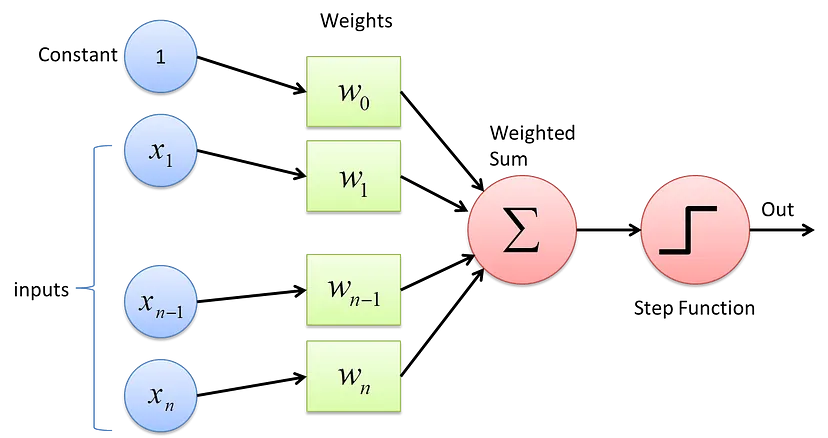
\includegraphics[scale=0.4]{figuras/perceptron.png}
    \caption{Perceptron Architecture. Font: \emph{Towards Data Science\footnotemark}. \label{fig:perceptron}}
\end{figure}
\footnotetext{https://towardsdatascience.com/what-the-hell-is-perceptron-626217814f53}

Where the weights \(w_i\) for \(i \in \{0, 1, \cdots, n\}\) are trainable parameters and the step function can be defined as \(\sigma \colon \mathbb{R} \to \{0, 1\}\) such that

\[\sigma(x) = 
\begin{cases}
    1 & \text{ if } x \geq 0 \\
    0 & \text{ if } x < 0.
\end{cases}\]

Therefore, the Perceptron model can be defined as the function \(f \colon \mathbb{R}^n \to \{0, 1\}\) where

\[f(x) = \sigma(w_0 + \sum_{i = 1}^{n} w_i x_i).\]

The Perceptron model updates its parameters using each sample \((x, y)\) of the dataset with the rule

\[w_i^{t + 1} = w_i^t + \eta \; (y - f(x)) x_i\]
for \(i \in \{1, \cdots, n\}\) and

\[w_0^{t + 1} = w_0^t + \eta \; (y - f(x)),\]
where \(\eta\) is the \emph{learning rate} hyperparameter and \(t\) is the update iteration number.

As a linear model, the Perceptron can only model linear problems. 
\section{Convolutional Neural Networks}
\label{sec:convolutions}

\lipsum[5-6]





%%%%%%%%%%%%%%%%%%%%%%%%%%%% APÊNDICES E ANEXOS %%%%%%%%%%%%%%%%%%%%%%%%%%%%%%%%

%%%% Apêndices %%%%

\cleardoublepage

\pagestyle{appendix}

\appendix

% \addappheadtotoc acrescenta a palavra "Apêndice" ao sumário; se
% só há apêndices, sem anexos, provavelmente não é necessário.
\addappheadtotoc

%!TeX root=../tese.tex
%("dica" para o editor de texto: este arquivo é parte de um documento maior)
% para saber mais: https://tex.stackexchange.com/q/78101

\chapter{Perguntas frequentes sobre o modelo}

\begin{itemize}

\item \textbf{Não consigo decorar tantos comandos!}\\
Use a colinha que é distribuída juntamente com este modelo (\url{gitlab.com/ccsl-usp/modelo-latex/raw/main/pre-compilados/colinha.pdf?inline=false}).

\item \textbf{Estou tendo problemas com caracteres acentuados.}\\
Versões modernas de \LaTeX{} usam UTF-8, mas arquivos antigos podem usar outras codificações (como ISO-8859-1, também conhecido como latin1 ou Windows-1252). Nesses casos, use \textsf{\textbackslash{}usepackage[latin1]\{inputenc\}} no preâmbulo do documento. Você também pode representar os caracteres acentuados usando comandos \LaTeX{}: \textsf{\textbackslash\textquotesingle{}a} para á, \textsf{\textbackslash{}c\{c\}} para cedilha etc., independentemente da codificação usada no texto\footnote{Você pode consultar os comandos desse tipo mais comuns em \url{en.wikibooks.org/wiki/LaTeX/Special_Characters}. Observe que a dica sobre o pingo do i \emph{não} é mais válida atualmente; basta usar \textsf{\textbackslash\textquotesingle{}i}.}.

\item \textbf{É possível resumir o nome das seções/capítulos que aparece no topo das páginas e no sumário?}\\
Sim, usando a sintaxe \textsf{\textbackslash{}section[mini-titulo]\{titulo enorme\}}. Isso é especialmente útil nas legendas (\textit{captions}\index{Legendas}) das figuras e tabelas, que muitas vezes são demasiadamente longas para a lista de figuras/tabelas.

\item \textbf{Existe algum programa para gerenciar referências em formato bibtex?}\\
Sim, há vários. Uma opção bem comum é o JabRef; outra é usar Zotero\index{Zotero} ou Mendeley\index{Mendeley} e exportar os dados deles no formato .bib.

\item \textbf{Posso usar pacotes \LaTeX{} adicionais aos sugeridos?}\\
Com certeza! Você pode modificar os arquivos o quanto desejar, o modelo serve só como uma ajuda inicial para o seu trabalho.

\end{itemize}

\par

%%%% Anexos %%%%

\cleardoublepage

\pagestyle{appendix} % repete o anterior, caso você não use apêndices

\annex

% \addappheadtotoc acrescenta a palavra "Anexo" ao sumário; se
% só há anexos, sem apêndices, provavelmente não é necessário.
\addappheadtotoc

% %!TeX root=../tese.tex
%("dica" para o editor de texto: este arquivo é parte de um documento maior)
% para saber mais: https://tex.stackexchange.com/q/78101

\chapter{As packages \pkg{imegoodies} e \pkg{imelooks}}
\label{ann:imegoodlooks}

Este modelo inclui as \textit{packages} \pkg{imegoodies} e \pkg{imelooks},
que você pode querer usar em outros documentos \LaTeX.

\pkg{imegoodies} inclui um grande número de \textit{packages} que são
comumente usadas e bastante úteis. Em geral, você pode incluí-la em seus
documentos sem que isso cause problemas de compatibilidade. Se, no
entanto, algo não funcionar, você pode editar o arquivo para eliminar
a \textit{package} responsável pelo problema se ela não for necessária.
\pkg{imegoodies} ainda inclui vários comentários explicativos sobre as
\textit{packages} carregadas.

\pkg{imelooks} também inclui um grande número de \textit{packages}, mas
estas são relacionadas mais explicitamente à aparência do documento
(fontes, cores, margens etc.). Você também pode utilizá-la em outros
documentos se quiser se aproximar da aparência deste modelo. \pkg{imelooks}
reconhece diversos parâmetros que ativam/desativam aspectos específicos:

\begin{itemize}
  \item \cmd{fonts} carrega as fontes deste modelo (libertinus e
        sourcecodepro), além de outros pequenos ajustes relacionados.
        Esta opção é sempre ativada por padrão; para desativá-la, use
        \cmd{nofonts}

  \item \cmd{spacing} utiliza os espaçamentos definidos neste modelo (margens,
        espaço entre parágrafos, indentação da primeira linha do parágrafo
        etc.). Esta opção é sempre ativada por padrão; para desativá-la, use
        \cmd{nospacing}

  \item \cmd{captions} e \cmd{footnotes} fazem respectivamente as legendas
        (das figuras e tabelas) e as notas de rodapé de acordo com este modelo.
        Estas opções são sempre ativadas por padrão; para desativá-las, use
        \cmd{nocaptions} e \cmd{nofootnotes}

  \item \cmd{autohttp} acrescenta o prefixo \cmd{http://} a URLs criadas
        com \ltxcmd{url} que não incluam o \textit{schema}. Esta opção é
        sempre ativada por padrão; para desativá-la, use \cmd{noautohttp}

  \item \cmd{hidelinks}, \cmd{borderlinks} e \cmd{colorlinks} definem a
        aparência dos hiperlinks. \cmd{hidelinks} faz os hiperlinks sem
        nenhuma formatação especial; \cmd{borderlinks} faz os hiperlinks
        serem envidos por um quadrado colorido (apenas na tela; o quadrado
        não é impresso); \cmd{colorlinks} faz o texto dos hiperlinks ser
        colorido. A opção \cmd{colorlinks} é sempre ativada por padrão

  \item \cmd{biblatex} carrega a \textit{package} \cmd{biblatex} e os
        estilos bibliográficos deste modelo. Esta opção é sempre ativada
        por padrão; para desativá-la, use \cmd{nobiblatex}
  \item \cmd{raggedbib} faz a bibliografia (com \cmd{biblatex}) ser
        formatada com alinhamento à esquerda ao invés de justificado.
        Esta opção é sempre ativada por padrão, exceto quando o estilo
        bibliográfico é \cmd{plainnat-ime} (usado nas teses); para
        desativá-la, use \cmd{noraggedbib}; para ativá-la incondicionalmente,
        use \cmd{raggedbib}
  \item \cmd{bibstyle=?} selectiona um estilo bibliográfico específico.
        O estilo padrão é \cmd{numeric}, exceto em pôsteres e apresentações
        (\cmd{beamer-ime}) e \textit{reports} (\cmd{plainnat-ime})

  \item \cmd{listings} carrega a \textit{package} \cmd{listings} e diversas
        configurações relacionadas usadas neste modelo. Esta opção é
        sempre ativada por padrão; para desativá-la, use \cmd{nolistings}

  \item \cmd{greeny}, \cmd{bluey}, \cmd{sandy} ativam esquemas de cores
        diferentes para pôsteres e apresentações (o padrão é \cmd{bluey})

  \item \cmd{beamer} \textbf{des}ativa algumas \textit{packages} que
        são incompatíveis com a classe \cmd{beamer} (note que as opções
        \cmd{slides} e \cmd{presentation}, discutidas abaixo, já fazem isso)

  \item \cmd{presentation} (ou \cmd{slides}) e \cmd{poster} ativam as
        opções relevantes para, respectivamente, apresentações com
        \cmd{beamer} ou pôsteres com \cmd{tcolorbox}

  \item \cmd{report} ativa as opções relevantes para documentos com
        capítulos (cabeçalhos das páginas, características do sumário etc.)

  \item \cmd{thesis} ativa a opção \cmd{report} e também define o que é
        necessário para a geração da capa das teses de acordo com este modelo

  \item \cmd{resumoabstract} define os comandos \cmd{resumo} e \cmd{abstract}
        de acordo com este modelo. Esta opção é ativada por padrão com
        \cmd{report}; para desativá-la, use \cmd{noresumoabstract}

  \item \cmd{brazilian} verifica se a língua portuguesa está ativa no
        documento e, em caso negativo, gera um erro. Esta opção é
        ativada por padrão com a opção \cmd{thesis}; para desativá-la,
        use \cmd{nobrazilian}
\end{itemize}
  % crashando aqui
\par
% %!TeX root=../tese.tex
%("dica" para o editor de texto: este arquivo é parte de um documento maior)
% para saber mais: https://tex.stackexchange.com/q/78101

\chapter{Código-fonte e pseudocódigo}
\label{ap:pseudocode}

Com a \textit{package} \textsf{listings}, programas podem ser inseridos
diretamente no arquivo, como feito no caso do Programa~\ref{prog:java},
ou importados de um arquivo externo com o comando
\textsf{\textbackslash{}lstinputlisting}, como no caso
do Programa~\ref{prog:mdcinput}.

% O exemplo foi copiado da documentação de algorithmicx
\begin{program}
  \lstinputlisting[
    language=pseudocode,
    style=pseudocode,
    style=wider,
    functions={},
    specialidentifiers={},
  ]
  {conteudo/euclid.psc}

  \caption{Máximo divisor comum (arquivo importado).\label{prog:mdcinput}}
\end{program}

Trechos de código curtos (menores que uma página) podem ou não ser
incluídos como \textit{floats}; trechos longos necessariamente incluem
quebras de página e, portanto, não podem ser \textit{floats}. Com
\textit{floats}, a legenda e as linhas separadoras são colocadas pelo
comando \textsf{\textbackslash{}begin\{program\}}; sem eles, utilize o
ambiente \textsf{programruledcaption} (atenção para a colocação do
comando \textsf{\textbackslash{}label\{\}}, dentro da legenda), como
no Programa~\ref{prog:mdc}\footnote{\textsf{listings} oferece alguns
recursos próprios para a definição de \textit{floats} e legendas, mas
neste modelo não os utilizamos.}:

\begin{programruledcaption}{Máximo divisor comum (em português).\label{prog:mdc}}
  \begin{lstlisting}[
    language={[brazilian]pseudocode},
    style=pseudocode,
    style=wider,
    functions={},
    specialidentifiers={},
  ]
      funcao euclides(a, b) // O máximo divisor comum de \textbf{a} e \textbf{b}
          r := a $\bmod$ b
	  enquanto r != 0 // Atingimos a resposta se \textbf{r} é zero
              a := b
              b := r
              r := a $\bmod$ b
          fim
	  devolva b // O máximo divisor comum é \textbf{b}
      fim
  \end{lstlisting}
\end{programruledcaption}

Além do suporte às várias linguagens incluídas em \textsf{listings},
este modelo traz uma extensão para permitir o uso de pseudocódigo,
útil para a descrição de algoritmos em alto nível. Ela oferece
diversos recursos:

\begin{itemize}

    \item Comentários seguem o padrão de C++ (\lstinline{//} e
          \lstinline{/* ... */}), mas o delimitador é impresso
          como ``$\triangleright$''.

    \item ``:='', ``<>'', ``<='', ``>='' e ``!='' são substituídos
          pelo símbolo matemático adequado.

    \item É possível acrescentar palavras-chave além de ``if'', ``and''
          etc. com a opção ``\textsf{morekeywords=\{pchave1,\linebreak[0]{}pchave2\}}''
          (para um trecho de código específico) ou com o comando
          \textsf{\textbackslash{}lstset\{morekeywords=\linebreak[0]{}\{pchave1,pchave2\}\}}
          (como comando de configuração geral).

    \item É possível usar pequenos trechos de código, como nomes de variáveis,
          dentro de um parágrafo normal com \textsf{\textbackslash{}lstinline\{blah\}}.

    \item ``\$\dots\$'' ativa o modo matemático em qualquer lugar.

    \item Outros comandos \LaTeX{} funcionam apenas em comentários; fora, a
          linguagem simula alguns pré-definidos (\textsf{\textbackslash{}textit\{\}},
          \textsf{\textbackslash{}texttt\{\}} etc.).

    \item O comando \textsf{\textbackslash{}label} também funciona em
          comentários; a referência correspondente (\textsf{\textbackslash{}ref})
          indica o número da linha de código. Se quiser usá-lo numa linha sem
          comentários, use \lstinline{///}~\textsf{\textbackslash{}label\{blah\}};
          ``\lstinline{///}'' funciona como \lstinline{//}, permitindo
          a inserção de comandos \LaTeX{}, mas não imprime o delimitador
          (\ensuremath{\triangleright}).

    \item Para suspender a formatação automática, use \textsf{\textbackslash{}noparse\{blah\}}.

    \item Para forçar a formatação de um texto como função, identificador,
          palavra-chave ou comentário, use \textsf{\textbackslash{}func\{blah\}},
          \textsf{\textbackslash{}id\{blah\}}, \textsf{\textbackslash{}kw\{blah\}} ou
          \textsf{\textbackslash{}comment\{blah\}}.

    \item Palavras-chave dentro de comentários não são formatadas
          automaticamente; se necessário, use \textsf{\textbackslash{}func\{\}},
          \textsf{\textbackslash{}id\{\}} etc. ou comandos \LaTeX{} padrão.

    \item As palavras ``Program'', ``Procedure'' e ``Function'' têm formatação
          especial e fazem a palavra seguinte ser formatada como função.
          Funções em outros lugares \emph{não} são detectadas automaticamente;
          use \textsf{\textbackslash{}func\{\}}, a opção ``\textsf{functions=\{func1,func2\}}''
          ou o comando ``\textsf{\textbackslash{}lstset\{functions=\{func1,func2\}\}}''
          para que elas sejam detectadas.

    \item Além de funções, palavras-chave, strings, comentários e
          identificadores, há ``\textsf{specialidentifiers}''. Você pode
          usá-los com \textsf{\textbackslash{}specialid\{blah\}}, com a opção
          ``\textsf{specialidentifiers=\{id1,id2\}}'' ou com o comando
          ``\textsf{\textbackslash{}lstset\{specialidentifiers=\{id1,id2\}\}}''.

\end{itemize}


  % crashando aqui também
\par

%%%%%%%%%%%%%%% SEÇÕES FINAIS (BIBLIOGRAFIA E ÍNDICE REMISSIVO) %%%%%%%%%%%%%%%%

% O comando backmatter desabilita a numeração de capítulos.
\backmatter

\pagestyle{backmatter}

% Espaço adicional no sumário antes das referências / índice remissivo
\addtocontents{toc}{\vspace{2\baselineskip plus .5\baselineskip minus .5\baselineskip}}

% A bibliografia é obrigatória

\printbibliography[
  title=\refname\label{sec:bib}, % "Referências", recomendado pela ABNT
  %title=\bibname\label{sec:bib}, % "Bibliografia"
  heading=bibintoc, % Inclui a bibliografia no sumário
]

\end{document}